\section{\textit{Entity Relationship Diagram}}

Berikut adalah gambaran kasar dari diagram relasi entitas pada sistem tiket yang menjadi bahasan pada penelitian ini:

\begin{figure}[htbp]
    \centering
    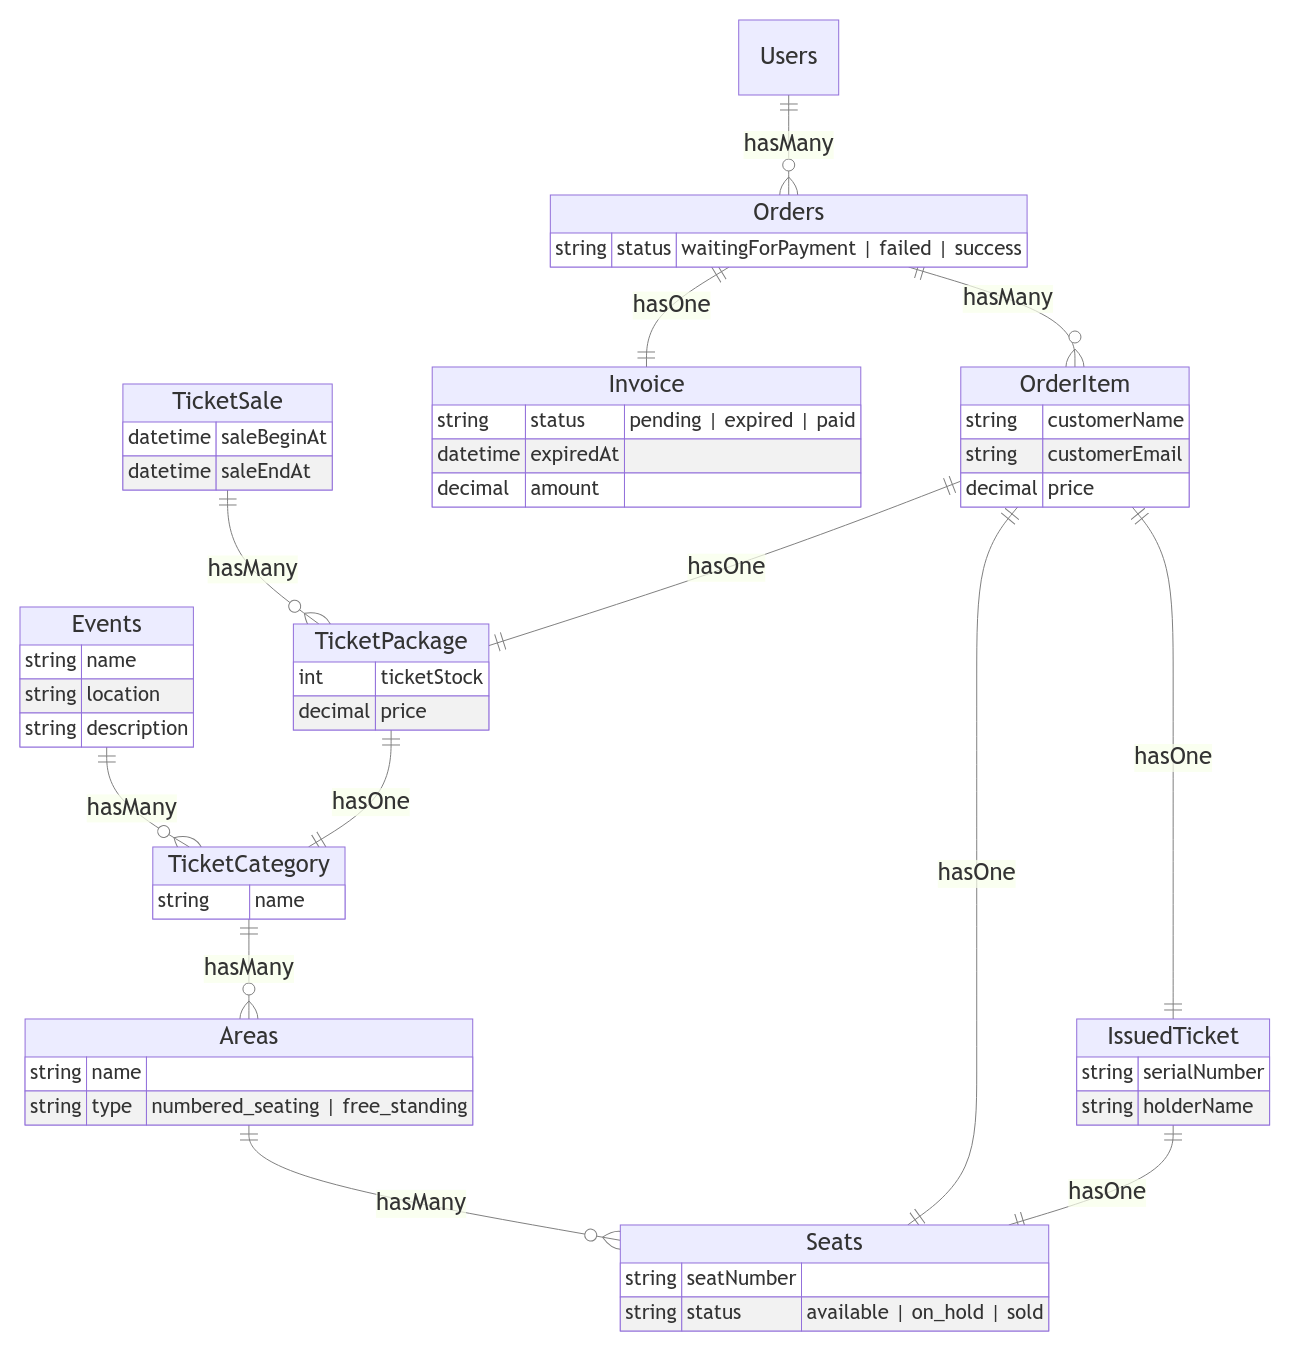
\includegraphics[width=1\textwidth]{resources/appendix/erd.png}
    \caption{ERD Sistem Tiket}
    \label{fig:ticket-system-erd-proposal}
\end{figure}

Berikut adalah pembagian entitas berdasarkan layanan:

\begingroup
\begin{longtable}{|p{0.3\textwidth}|p{0.7\textwidth}|}
    \caption{Kebutuhan Non-Fungsional Sistem Tiket}                                                                                \\
    \hline
    \textbf{Layanan} & \textbf{Entitas}                                                                                            \\
    \hline
    \endfirsthead

    \multicolumn{2}{|l|}{\tablename\ \thetable\ -- \textit{Lanjutan dari halaman sebelumnya}}                                      \\
    \hline
    \textbf{Layanan} & \textbf{Entitas}                                                                                            \\
    \hline
    \endhead

    \hline
    \multicolumn{2}{|r|}{\textit{Dilanjutkan ke halaman berikutnya}}                                                               \\
    \endfoot

    \hline
    \endlastfoot

    \hline
    Tiket            & Events, TicketCategory, Areas, Seats, TicketSale, \linebreak TicketPackage, Orders, OrderItem, IssuedTicket \\
    \hline
    \hline
    Pengguna         & Users                                                                                                       \\
    \hline
    \hline
    Pembayaran       & Invoice                                                                                                     \\
    \hline
\end{longtable}
\endgroup